\documentclass[11pt]{article}
\input{headers05}

\usepackage{fancyhdr}   
\pagestyle{fancy}      
\lhead{CS 355, FALL 2020}               
\rhead{Name: Chris Cohen}

\usepackage[strict]{changepage}  
\newcommand{\nextoddpage}{\checkoddpage\ifoddpage{\ \newpage\ \newpage}\else{\ \newpage}\fi}  


\begin{document}

\title{Homework 5}

\date{}

\maketitle 

\thispagestyle{fancy}  
\pagestyle{fancy}      




\begin{enumerate}



%%%%%%%%%%%%%%%%%%%%%%%%%%%%%%%%%%%%%%%%%%%%%%%%%%
%%%%%%%%%%%% PROBLEM 1 %%%%%%%%%%%%%%%%%%%%%%%%%%%%
%%%%%%%%%%%%%%%%%%%%%%%%%%%%%%%%%%%%%%%%%%%%%%%%%%%
\item {\bfseries Stretching PRG Output.} (10 points)
Suppose we are given a length-doubling PRG $G$ such that 
$$G:\{0,1\}^B \rightarrow \{0,1\}^{2B}$$
Using $G$, construct a new PRG $G'$ such that 
$$G': \{0,1\}^B \rightarrow \{0,1\}^{2020B}$$

({\footnotesize Remark: We do not need a security proof. 
You should only use the PRG $G$ to construct the new PRG $G'$. 
In particular, you should not use any other cryptographic primitive like one-way function etc.}%
)

%%%%% ANSWER %%%%%
    {\bfseries
      $G'$ should start off by running a bit string B through $G$. From there, it should continually feed the lower B bits from the newly generated bit string of length 2B into G until the total length is 2020B. Executing G once would give you a bit string of length 2B. Twice would give you length 3B, three times would give you length 4B, etc. If you execute G a total of 2019 times, then the length of the final bit string would be 2020B. An illustration is provided below. \newline
      %%%%% FROM https://www.mathcha.io/editor %%%%%

\tikzset{every picture/.style={line width=0.75pt}} %set default line width to 0.75pt

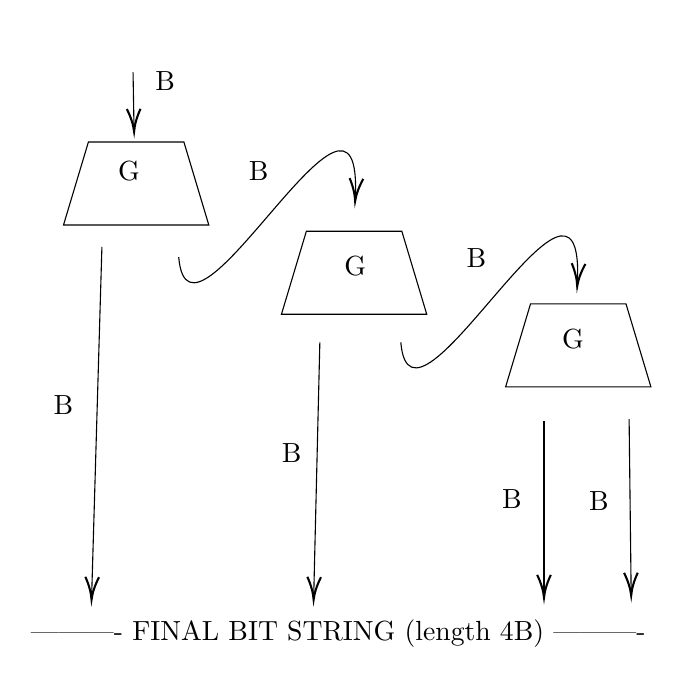
\begin{tikzpicture}[x=0.75pt,y=0.75pt,yscale=-1,xscale=1]
%uncomment if require: \path (0,300); %set diagram left start at 0, and has height of 300

%Shape: Trapezoid [id:dp026330063344337074]
\draw   (104,81) -- (116,41) -- (162,41) -- (174,81) -- cycle ;
%Shape: Trapezoid [id:dp7703141904630679]
\draw   (209,124) -- (221,84) -- (267,84) -- (279,124) -- cycle ;
%Shape: Trapezoid [id:dp856778076812458]
\draw   (317,159) -- (329,119) -- (375,119) -- (387,159) -- cycle ;
%Straight Lines [id:da25343126364307733]
\draw    (137.5,7.5) -- (137.96,34) ;
\draw [shift={(138,36)}, rotate = 268.99] [color={rgb, 255:red, 0; green, 0; blue, 0 }  ][line width=0.75]    (10.93,-3.29) .. controls (6.95,-1.4) and (3.31,-0.3) .. (0,0) .. controls (3.31,0.3) and (6.95,1.4) .. (10.93,3.29)   ;
%Straight Lines [id:da1289027369849567]
\draw    (122.5,91.5) -- (117.56,259.5) ;
\draw [shift={(117.5,261.5)}, rotate = 271.68] [color={rgb, 255:red, 0; green, 0; blue, 0 }  ][line width=0.75]    (10.93,-3.29) .. controls (6.95,-1.4) and (3.31,-0.3) .. (0,0) .. controls (3.31,0.3) and (6.95,1.4) .. (10.93,3.29)   ;
%Straight Lines [id:da6734929502520619]
\draw    (227.5,137.5) -- (224.55,259.5) ;
\draw [shift={(224.5,261.5)}, rotate = 271.39] [color={rgb, 255:red, 0; green, 0; blue, 0 }  ][line width=0.75]    (10.93,-3.29) .. controls (6.95,-1.4) and (3.31,-0.3) .. (0,0) .. controls (3.31,0.3) and (6.95,1.4) .. (10.93,3.29)   ;
%Straight Lines [id:da4159392017215253]
\draw    (335.5,175.5) -- (335.5,258.5) ;
\draw [shift={(335.5,260.5)}, rotate = 270] [color={rgb, 255:red, 0; green, 0; blue, 0 }  ][line width=0.75]    (10.93,-3.29) .. controls (6.95,-1.4) and (3.31,-0.3) .. (0,0) .. controls (3.31,0.3) and (6.95,1.4) .. (10.93,3.29)   ;
%Straight Lines [id:da8820092940988289]
\draw    (376.5,174.5) -- (377.48,257.5) ;
\draw [shift={(377.5,259.5)}, rotate = 269.33] [color={rgb, 255:red, 0; green, 0; blue, 0 }  ][line width=0.75]    (10.93,-3.29) .. controls (6.95,-1.4) and (3.31,-0.3) .. (0,0) .. controls (3.31,0.3) and (6.95,1.4) .. (10.93,3.29)   ;
%Curve Lines [id:da9419391578140921]
\draw    (159.5,96.5) .. controls (164.48,154.21) and (248.65,-13.81) .. (244.57,68.24) ;
\draw [shift={(244.5,69.5)}, rotate = 273.37] [color={rgb, 255:red, 0; green, 0; blue, 0 }  ][line width=0.75]    (10.93,-3.29) .. controls (6.95,-1.4) and (3.31,-0.3) .. (0,0) .. controls (3.31,0.3) and (6.95,1.4) .. (10.93,3.29)   ;
%Curve Lines [id:da6965331206884073]
\draw    (266.5,137.5) .. controls (271.48,195.21) and (355.65,27.19) .. (351.57,109.24) ;
\draw [shift={(351.5,110.5)}, rotate = 273.37] [color={rgb, 255:red, 0; green, 0; blue, 0 }  ][line width=0.75]    (10.93,-3.29) .. controls (6.95,-1.4) and (3.31,-0.3) .. (0,0) .. controls (3.31,0.3) and (6.95,1.4) .. (10.93,3.29)   ;

% Text Node
\draw (87,270) node [anchor=north west][inner sep=0.75pt]   [align=left] {---------- FINAL BIT STRING (length 4B) ----------};
% Text Node
\draw (147,6) node [anchor=north west][inner sep=0.75pt]   [align=left] {B};
% Text Node
\draw (356,208) node [anchor=north west][inner sep=0.75pt]   [align=left] {B};
% Text Node
\draw (314,207) node [anchor=north west][inner sep=0.75pt]   [align=left] {B};
% Text Node
\draw (297,91) node [anchor=north west][inner sep=0.75pt]   [align=left] {B};
% Text Node
\draw (208,185) node [anchor=north west][inner sep=0.75pt]   [align=left] {B};
% Text Node
\draw (192,49) node [anchor=north west][inner sep=0.75pt]   [align=left] {B};
% Text Node
\draw (98,162) node [anchor=north west][inner sep=0.75pt]   [align=left] {B};
% Text Node
\draw (129,49) node [anchor=north west][inner sep=0.75pt]   [align=left] {G};
% Text Node
\draw (238,95) node [anchor=north west][inner sep=0.75pt]   [align=left] {G};
% Text Node
\draw (343,130) node [anchor=north west][inner sep=0.75pt]   [align=left] {G};


\end{tikzpicture}

Basically, using the above method, after executing $G$ 2019 times, you will have a bit string of length 2020B.

    }
%%%%%%%%%%%%%%%%%%
     \newpage


%%%%%%%%%%%%%%%%%%%%%%% %%%%%%%%%%%%%%%%%%%%%%%%%%%%
%%%%%%%%% PROBLEM 2 %%%%%%%%%%%%%%%%%%%%%%%%%%%%
%%%%%%%%%%%%%%%%%%%%%%%%%%%%%%%%%%%%%%%%%%%%%%%%%%%

\item {\bfseries New Pseudorandom Function Family.} (7+8+10) 
  Let $G$ be a length-doubling PRG $G\colon\zo^B\to\zo^{2B}$. 
  Recall the basic  GGM PRF construction presented below. 
   \begin{boxedalgo}
 \begin{itemize}
     \item  Define $G(x) = (G_0(x), G_1(x))$ where $G_0,G_1 : \{0,1\}^B \rightarrow \{0,1\}^B$
%    \item Let $G' : \{0,1\}^B \rightarrow \{0,1\}^n$ be a PRG. 
    \item  We define $g_{\pred{id}}(x_1,x_2,\ldots x_n)$ as $G_{x_n}(\ldots G_{x_2}(G_{x_1}(\pred{id})) \ldots )$ \\where $\pred{id} \xleftarrow[]{\$} \zo^B$.
 \end{itemize}
  \end{boxedalgo}
  Recall that in the class we studied that $g_{\pred{id}}$ is a PRF family for $\zo^n\to\zo^B$, for a fixed value of $n$ when the key $\pred{id}$ is picked uniformly at random from the set $\zo^B$. 

  \begin{enumerate}
   \item (7 points) Why is the above-mentioned GGM construction not a pseudorandom function family from the domain $\zo^*$ to the range $\zo^B$? (Note that $\{0,1\}^{*}$ means that the length of the input to the PRF is arbitrary) \newline 
%%%%% ANSWER %%%%%
    {\bfseries

      Let's consider the example inputs $3 (11)$, $6 (110)$, and $12 (1100)$. Note that they all have a differing number of bits, but the first two bits are identical among the three. Executing GGM construction on the inputs result in the following: \newline




\tikzset{every picture/.style={line width=0.75pt}} %set default line width to 0.75pt        

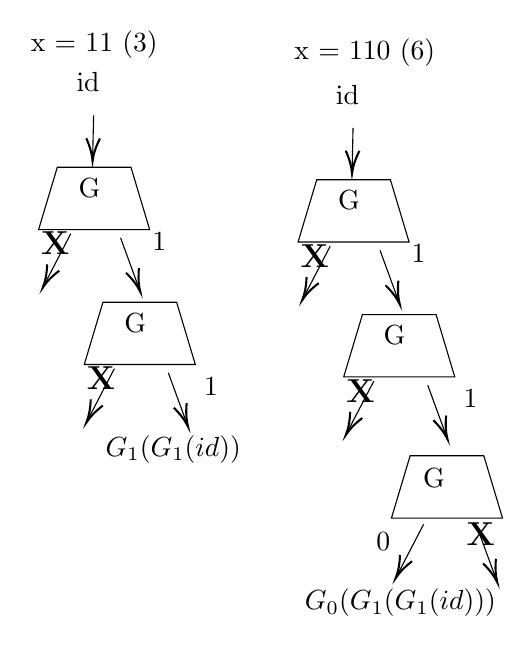
\begin{tikzpicture}[x=0.75pt,y=0.75pt,yscale=-1,xscale=1]
%uncomment if require: \path (0,483); %set diagram left start at 0, and has height of 483

%Shape: Trapezoid [id:dp2852104231671544] 
\draw   (45,120) -- (54,90) -- (89.5,90) -- (98.5,120) -- cycle ;
%Shape: Trapezoid [id:dp165141673263979] 
\draw   (67,185) -- (76,155) -- (111.5,155) -- (120.5,185) -- cycle ;
%Straight Lines [id:da29030255403190575] 
\draw    (107.5,189) -- (116.31,213.12) ;
\draw [shift={(117,215)}, rotate = 249.93] [color={rgb, 255:red, 0; green, 0; blue, 0 }  ][line width=0.75]    (10.93,-3.29) .. controls (6.95,-1.4) and (3.31,-0.3) .. (0,0) .. controls (3.31,0.3) and (6.95,1.4) .. (10.93,3.29)   ;
%Straight Lines [id:da9510990729773141] 
\draw    (84.5,124) -- (93.31,148.12) ;
\draw [shift={(94,150)}, rotate = 249.93] [color={rgb, 255:red, 0; green, 0; blue, 0 }  ][line width=0.75]    (10.93,-3.29) .. controls (6.95,-1.4) and (3.31,-0.3) .. (0,0) .. controls (3.31,0.3) and (6.95,1.4) .. (10.93,3.29)   ;
%Straight Lines [id:da0037293976213679247] 
\draw    (60.5,122) -- (47.92,146.23) ;
\draw [shift={(47,148)}, rotate = 297.44] [color={rgb, 255:red, 0; green, 0; blue, 0 }  ][line width=0.75]    (10.93,-3.29) .. controls (6.95,-1.4) and (3.31,-0.3) .. (0,0) .. controls (3.31,0.3) and (6.95,1.4) .. (10.93,3.29)   ;
%Straight Lines [id:da8228080900603938] 
\draw    (81.5,187) -- (68.92,211.23) ;
\draw [shift={(68,213)}, rotate = 297.44] [color={rgb, 255:red, 0; green, 0; blue, 0 }  ][line width=0.75]    (10.93,-3.29) .. controls (6.95,-1.4) and (3.31,-0.3) .. (0,0) .. controls (3.31,0.3) and (6.95,1.4) .. (10.93,3.29)   ;
%Straight Lines [id:da28500051662317105] 
\draw    (71.5,65) -- (71.05,85) ;
\draw [shift={(71,87)}, rotate = 271.3] [color={rgb, 255:red, 0; green, 0; blue, 0 }  ][line width=0.75]    (10.93,-3.29) .. controls (6.95,-1.4) and (3.31,-0.3) .. (0,0) .. controls (3.31,0.3) and (6.95,1.4) .. (10.93,3.29)   ;
%Shape: Trapezoid [id:dp6325112610108554] 
\draw   (170,126) -- (179,96) -- (214.5,96) -- (223.5,126) -- cycle ;
%Shape: Trapezoid [id:dp25188600140982165] 
\draw   (192,191) -- (201,161) -- (236.5,161) -- (245.5,191) -- cycle ;
%Shape: Trapezoid [id:dp7252358609087375] 
\draw   (215,259) -- (224,229) -- (259.5,229) -- (268.5,259) -- cycle ;
%Straight Lines [id:da7972073805415487] 
\draw    (232.5,195) -- (241.31,219.12) ;
\draw [shift={(242,221)}, rotate = 249.93] [color={rgb, 255:red, 0; green, 0; blue, 0 }  ][line width=0.75]    (10.93,-3.29) .. controls (6.95,-1.4) and (3.31,-0.3) .. (0,0) .. controls (3.31,0.3) and (6.95,1.4) .. (10.93,3.29)   ;
%Straight Lines [id:da018853121174194687] 
\draw    (209.5,130) -- (218.31,154.12) ;
\draw [shift={(219,156)}, rotate = 249.93] [color={rgb, 255:red, 0; green, 0; blue, 0 }  ][line width=0.75]    (10.93,-3.29) .. controls (6.95,-1.4) and (3.31,-0.3) .. (0,0) .. controls (3.31,0.3) and (6.95,1.4) .. (10.93,3.29)   ;
%Straight Lines [id:da7054896933784254] 
\draw    (185.5,128) -- (172.92,152.23) ;
\draw [shift={(172,154)}, rotate = 297.44] [color={rgb, 255:red, 0; green, 0; blue, 0 }  ][line width=0.75]    (10.93,-3.29) .. controls (6.95,-1.4) and (3.31,-0.3) .. (0,0) .. controls (3.31,0.3) and (6.95,1.4) .. (10.93,3.29)   ;
%Straight Lines [id:da18444998536360768] 
\draw    (206.5,193) -- (193.92,217.23) ;
\draw [shift={(193,219)}, rotate = 297.44] [color={rgb, 255:red, 0; green, 0; blue, 0 }  ][line width=0.75]    (10.93,-3.29) .. controls (6.95,-1.4) and (3.31,-0.3) .. (0,0) .. controls (3.31,0.3) and (6.95,1.4) .. (10.93,3.29)   ;
%Straight Lines [id:da255539280729278] 
\draw    (196.5,71) -- (196.05,91) ;
\draw [shift={(196,93)}, rotate = 271.3] [color={rgb, 255:red, 0; green, 0; blue, 0 }  ][line width=0.75]    (10.93,-3.29) .. controls (6.95,-1.4) and (3.31,-0.3) .. (0,0) .. controls (3.31,0.3) and (6.95,1.4) .. (10.93,3.29)   ;
%Straight Lines [id:da9761312714264434] 
\draw    (256.5,264) -- (265.31,288.12) ;
\draw [shift={(266,290)}, rotate = 249.93] [color={rgb, 255:red, 0; green, 0; blue, 0 }  ][line width=0.75]    (10.93,-3.29) .. controls (6.95,-1.4) and (3.31,-0.3) .. (0,0) .. controls (3.31,0.3) and (6.95,1.4) .. (10.93,3.29)   ;
%Straight Lines [id:da6224568075589378] 
\draw    (230.5,262) -- (217.92,286.23) ;
\draw [shift={(217,288)}, rotate = 297.44] [color={rgb, 255:red, 0; green, 0; blue, 0 }  ][line width=0.75]    (10.93,-3.29) .. controls (6.95,-1.4) and (3.31,-0.3) .. (0,0) .. controls (3.31,0.3) and (6.95,1.4) .. (10.93,3.29)   ;

% Text Node
\draw (62,43) node [anchor=north west][inner sep=0.75pt]   [align=left] {id};
% Text Node
\draw (63,94) node [anchor=north west][inner sep=0.75pt]   [align=left] {G};
% Text Node
\draw (85,159) node [anchor=north west][inner sep=0.75pt]   [align=left] {G};
% Text Node
\draw (67,185) node [anchor=north west][inner sep=0.75pt]   [align=left] {\textbf{{\large X}}};
% Text Node
\draw (45,120) node [anchor=north west][inner sep=0.75pt]   [align=left] {\textbf{{\large X}}};
% Text Node
\draw (40,23) node [anchor=north west][inner sep=0.75pt]   [align=left] {x = 11 (3)};
% Text Node
\draw (98.5,120) node [anchor=north west][inner sep=0.75pt]   [align=left] {1};
% Text Node
\draw (123.5,190) node [anchor=north west][inner sep=0.75pt]   [align=left] {1};
% Text Node
\draw (187,49) node [anchor=north west][inner sep=0.75pt]   [align=left] {id};
% Text Node
\draw (188,100) node [anchor=north west][inner sep=0.75pt]   [align=left] {G};
% Text Node
\draw (210,165) node [anchor=north west][inner sep=0.75pt]   [align=left] {G};
% Text Node
\draw (229,234) node [anchor=north west][inner sep=0.75pt]   [align=left] {G};
% Text Node
\draw (192,191) node [anchor=north west][inner sep=0.75pt]   [align=left] {\textbf{{\large X}}};
% Text Node
\draw (170,126) node [anchor=north west][inner sep=0.75pt]   [align=left] {\textbf{{\large X}}};
% Text Node
\draw (167,27) node [anchor=north west][inner sep=0.75pt]   [align=left] {x = 110 (6)};
% Text Node
\draw (223.5,126) node [anchor=north west][inner sep=0.75pt]   [align=left] {1};
% Text Node
\draw (248.5,196) node [anchor=north west][inner sep=0.75pt]   [align=left] {1};
% Text Node
\draw (206.5,265) node [anchor=north west][inner sep=0.75pt]   [align=left] {0};
% Text Node
\draw (250,260) node [anchor=north west][inner sep=0.75pt]   [align=left] {\textbf{{\large X}}};
% Text Node
\draw (76,218) node [anchor=north west][inner sep=0.75pt]    {$G_{1}( G_{1}( id))$};
% Text Node
\draw (172,292) node [anchor=north west][inner sep=0.75pt]    {$G_{0}( G_{1}( G_{1}( id)))$};


\end{tikzpicture}

  As you can see, the beginning of these GGM constructions are identical (the first two bits 11). The output of $g_{id}(11) = G_1(G_1(id))$, and the output of $g_{id}(110) = G_0(G_1(G_1(id))$. Notice that the output of $g_{id}(110)$ is simply $G_0$ applied on the output of $g_{id}(11)$. This means that we can invert the PRG G, violating the security of the PRF Family. Since we know $G$ and $g_{id}(11)$, we can calculate $g_{id}(111)$. \newline

  Since the output no longer appears uniformly random, and can be predicted, we can conclude that the mentioned GGM Construction is NOT a PRFF.
    }
%%%%%%%%%%%%%%%%%%
     \newpage
  \item (8 points) Given a length-doubling PRG $G\colon\zo^B\to\zo^{2B}$, construct a PRF family from the domain $\zo^n$ to the range $\zo^{2020B}$. \newline 
  ({\footnotesize Remark: Again, in this problem, do not use any other cryptographic primitive like one-way function etc. You should only use the PRG $G$ in your proposed construction.}) \newline 
%%%%% ANSWER %%%%%
    {\bfseries

      To start, I will declare a few different variables: \newline
   \begin{boxedalgo}
 \begin{itemize}
      \item $id$ will be selected uniformly at random from the set $\{0,1\}^B$
      \item $x$ will be selected selected uniformly at random from the domain $\{0,1\}^{n}$
      \item $G' : \{0,1\}^B  \to \{0,1\}^{2020B}$, from Q1 (this only uses G).
 \end{itemize}
  \end{boxedalgo}
      Now, the GGM construction for the PRFF is detailed below: \newline




\tikzset{every picture/.style={line width=0.75pt}} %set default line width to 0.75pt

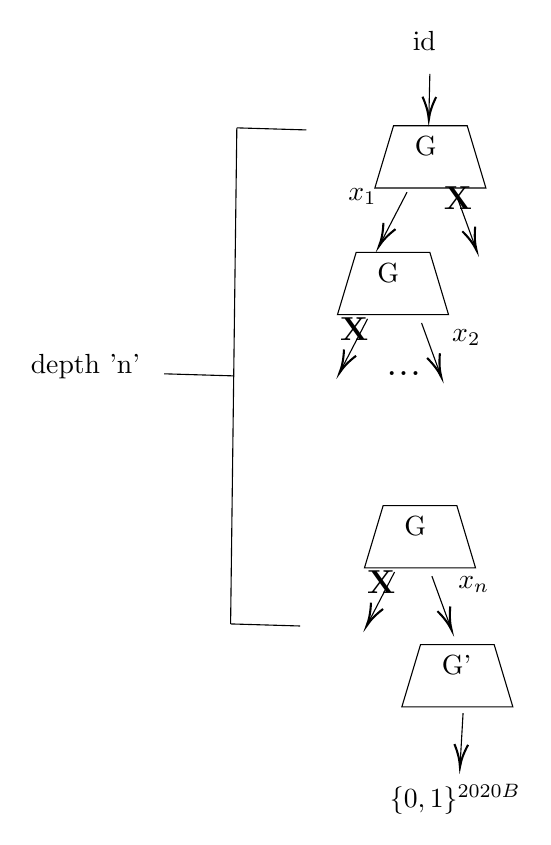
\begin{tikzpicture}[x=0.75pt,y=0.75pt,yscale=-1,xscale=1]
%uncomment if require: \path (0,411); %set diagram left start at 0, and has height of 411

%Shape: Trapezoid [id:dp2852104231671544]
\draw   (289,84) -- (298,54) -- (333.5,54) -- (342.5,84) -- cycle ;
%Shape: Trapezoid [id:dp165141673263979]
\draw   (271,145) -- (280,115) -- (315.5,115) -- (324.5,145) -- cycle ;
%Shape: Trapezoid [id:dp26205065292470864]
\draw   (284,267) -- (293,237) -- (328.5,237) -- (337.5,267) -- cycle ;
%Shape: Trapezoid [id:dp9053016549460027]
\draw   (302,334) -- (311,304) -- (346.5,304) -- (355.5,334) -- cycle ;
%Straight Lines [id:da29030255403190575]
\draw    (311.5,149) -- (320.31,173.12) ;
\draw [shift={(321,175)}, rotate = 249.93] [color={rgb, 255:red, 0; green, 0; blue, 0 }  ][line width=0.75]    (10.93,-3.29) .. controls (6.95,-1.4) and (3.31,-0.3) .. (0,0) .. controls (3.31,0.3) and (6.95,1.4) .. (10.93,3.29)   ;
%Straight Lines [id:da7860788752509089]
\draw    (316.5,271) -- (325.31,295.12) ;
\draw [shift={(326,297)}, rotate = 249.93] [color={rgb, 255:red, 0; green, 0; blue, 0 }  ][line width=0.75]    (10.93,-3.29) .. controls (6.95,-1.4) and (3.31,-0.3) .. (0,0) .. controls (3.31,0.3) and (6.95,1.4) .. (10.93,3.29)   ;
%Straight Lines [id:da9510990729773141]
\draw    (328.5,88) -- (337.31,112.12) ;
\draw [shift={(338,114)}, rotate = 249.93] [color={rgb, 255:red, 0; green, 0; blue, 0 }  ][line width=0.75]    (10.93,-3.29) .. controls (6.95,-1.4) and (3.31,-0.3) .. (0,0) .. controls (3.31,0.3) and (6.95,1.4) .. (10.93,3.29)   ;
%Straight Lines [id:da0037293976213679247]
\draw    (304.5,86) -- (291.92,110.23) ;
\draw [shift={(291,112)}, rotate = 297.44] [color={rgb, 255:red, 0; green, 0; blue, 0 }  ][line width=0.75]    (10.93,-3.29) .. controls (6.95,-1.4) and (3.31,-0.3) .. (0,0) .. controls (3.31,0.3) and (6.95,1.4) .. (10.93,3.29)   ;
%Straight Lines [id:da8228080900603938]
\draw    (285.5,147) -- (272.92,171.23) ;
\draw [shift={(272,173)}, rotate = 297.44] [color={rgb, 255:red, 0; green, 0; blue, 0 }  ][line width=0.75]    (10.93,-3.29) .. controls (6.95,-1.4) and (3.31,-0.3) .. (0,0) .. controls (3.31,0.3) and (6.95,1.4) .. (10.93,3.29)   ;
%Straight Lines [id:da6681042705492621]
\draw    (298.5,269) -- (285.92,293.23) ;
\draw [shift={(285,295)}, rotate = 297.44] [color={rgb, 255:red, 0; green, 0; blue, 0 }  ][line width=0.75]    (10.93,-3.29) .. controls (6.95,-1.4) and (3.31,-0.3) .. (0,0) .. controls (3.31,0.3) and (6.95,1.4) .. (10.93,3.29)   ;
%Straight Lines [id:da5253978309827989]
\draw    (331.5,337) -- (330.12,361) ;
\draw [shift={(330,363)}, rotate = 273.3] [color={rgb, 255:red, 0; green, 0; blue, 0 }  ][line width=0.75]    (10.93,-3.29) .. controls (6.95,-1.4) and (3.31,-0.3) .. (0,0) .. controls (3.31,0.3) and (6.95,1.4) .. (10.93,3.29)   ;
%Straight Lines [id:da8460909959823788]
\draw    (222.5,55) -- (219.5,294) ;
%Straight Lines [id:da7967658506445916]
\draw    (256,56) -- (222.5,55) ;
%Straight Lines [id:da1155834041490118]
\draw    (253,295) -- (219.5,294) ;
%Straight Lines [id:da12539749270882683]
\draw    (221,174.5) -- (187.5,173.5) ;
%Straight Lines [id:da28500051662317105]
\draw    (315.5,29) -- (315.05,49) ;
\draw [shift={(315,51)}, rotate = 271.3] [color={rgb, 255:red, 0; green, 0; blue, 0 }  ][line width=0.75]    (10.93,-3.29) .. controls (6.95,-1.4) and (3.31,-0.3) .. (0,0) .. controls (3.31,0.3) and (6.95,1.4) .. (10.93,3.29)   ;

% Text Node
\draw (306,7) node [anchor=north west][inner sep=0.75pt]   [align=left] {id};
% Text Node
\draw (307,58) node [anchor=north west][inner sep=0.75pt]   [align=left] {G};
% Text Node
\draw (289,119) node [anchor=north west][inner sep=0.75pt]   [align=left] {G};
% Text Node
\draw (293,171) node [anchor=north west][inner sep=0.75pt]   [align=left] {{\LARGE ...}};
% Text Node
\draw (302,241) node [anchor=north west][inner sep=0.75pt]   [align=left] {G};
% Text Node
\draw (320,308) node [anchor=north west][inner sep=0.75pt]   [align=left] {G'};
% Text Node
\draw (284,267) node [anchor=north west][inner sep=0.75pt]   [align=left] {\textbf{{\large X}}};
% Text Node
\draw (271,145) node [anchor=north west][inner sep=0.75pt]   [align=left] {\textbf{{\large X}}};
% Text Node
\draw (321,82) node [anchor=north west][inner sep=0.75pt]   [align=left] {\textbf{{\large X}}};
% Text Node
\draw (122,163) node [anchor=north west][inner sep=0.75pt]   [align=left] {depth 'n'};
% Text Node
\draw (295,370) node [anchor=north west][inner sep=0.75pt]    {$\{0,1\}^{2020B}$};
% Text Node
\draw (328,270) node [anchor=north west][inner sep=0.75pt]    {$x_{n}$};
% Text Node
\draw (325,151) node [anchor=north west][inner sep=0.75pt]    {$x_{2}$};
% Text Node
\draw (275,83) node [anchor=north west][inner sep=0.75pt]    {$x_{1}$};


\end{tikzpicture}


    }
%%%%%%%%%%%%%%%%%%
     \newpage
  \item (10 points) Consider the following function family $\{h_1,\dotsc,h_\alpha\}$ from the domain $\zo^*$ to the range $\zo^B$. 
    We define $h_{\pred{id}}(x) = g_{\pred{id}}(x , [\;\abs x\;]_2)$, for $\pred{id}\in\{1,2,\dotsc,\alpha\}$. 
    Show that $\{h_1,\dotsc,h_\alpha\}$ is \ul{not} a secure PRF from $\zo^*$ to the range $\zo^B$. 
    
    ({\footnotesize {\em Note}: The expression $[\;\abs x\;]_2$ represents the length of $x$ in $n$-bit binary expression. ($n$ denotes the length of $x$)}) \newline 
%%%%% ANSWER %%%%%
    {\bfseries

    For this, I will again use the example of $x=3 (11)$ vs $x=6 (110)$. Recall that the binary representation of $3$ has $2$ bits, and the binary representation of $6$ has $3$ bits. \newline

    $h_{id}(x) = g_{id}(x, [\;\abs x\;]_2)$ \newline
    $h_{id}(11) = g_{id}(11,10)$ \newline
    $h_{id}(110) = g_{id}(110,11)$ \newline

  The fact that the domain for this function family takes inputs of different lengths allows us to compromise the security of $g_{id}$, in a similar fashion to 2a and 3. \newline

    If you keep testing inputs, it becomes clear that, for all 2-bit numbers, the second argument of $g_{id}$ will be $10$, $11$ for all 3-bit numbers, $100$ for all 4-bit numbers, and so on. This means that the output is not completely independent of the input, which violates the definition of a PRFF. \newline
    }
%%%%%%%%%%%%%%%%%%
     \newpage
  \end{enumerate} 
  



%%%%%%%%%%%%%%%%%%%%%%% %%%%%%%%%%%%%%%%%%%%%%%%%%%%
%%%%%%%%% PROBLEM 3 %%%%%%%%%%%%%%%%%%%%%%%%%%%%
%%%%%%%%%%%%%%%%%%%%%%%%%%%%%%%%%%%%%%%%%%%%%%%%%%%

\item {\bfseries Variant of Pseudorandom Function Family.} (15 points)
  Let $G$ be a length-doubling PRG $G\colon\zo^B\to\zo^{2B}$ and $G' : \{0,1\}^B \rightarrow \{0,1\}^T$ be a PRG where $T\geq B$. 
  The following construction is suggested to construct a PRF family from $\{0,1\}^* \rightarrow \{0,1\}^T$. 
  (Note that $\{0,1\}^{*}$ means that the length of the input to the PRF is arbitrary) 
   \begin{boxedalgo}
 \begin{itemize}
     \item Define $G(x) = (G_0(x), G_1(x))$ where $G_0,G_1 : \{0,1\}^B \rightarrow \{0,1\}^B$
   \item Let $G' : \{0,1\}^B \rightarrow \{0,1\}^T$ be a PRG. 
    \item We define $g_{\pred{id}}(x_1,x_2,\ldots x_n)$ as $G'(G_{x_n}(\ldots G_{x_2}(G_{x_1}(\pred{id})) \ldots ))$ \\where $\pred{id} \xleftarrow[]{\$} \zo^B$.
 \end{itemize}
  \end{boxedalgo}
  
 % In this problem, we shall generalize the GGM PRF construction in two ways. 
  %\begin{enumerate}
   %\item 
 Prove that the above-mentioned PRF construction is \ul{not} secure when $G'=G$. (Note that when $G'=G$, then $T=2B$). 
   %\end{enumerate} 
  

%%%%% ANSWER %%%%%
    {\bfseries

    Imagine inputs $3 (11)$, $6 (110)$, and $7 (111)$. Note that three only has 2 bits, and all three numbers start with the bits $11$. This means that the evaluation of GGM up to the first 2 bits deep will be identical for all three inputs. Also note that we are fixing the function $id$ chosen from the PRFF. Evaluating GGM Construction results in the following:


\tikzset{every picture/.style={line width=0.75pt}} %set default line width to 0.75pt

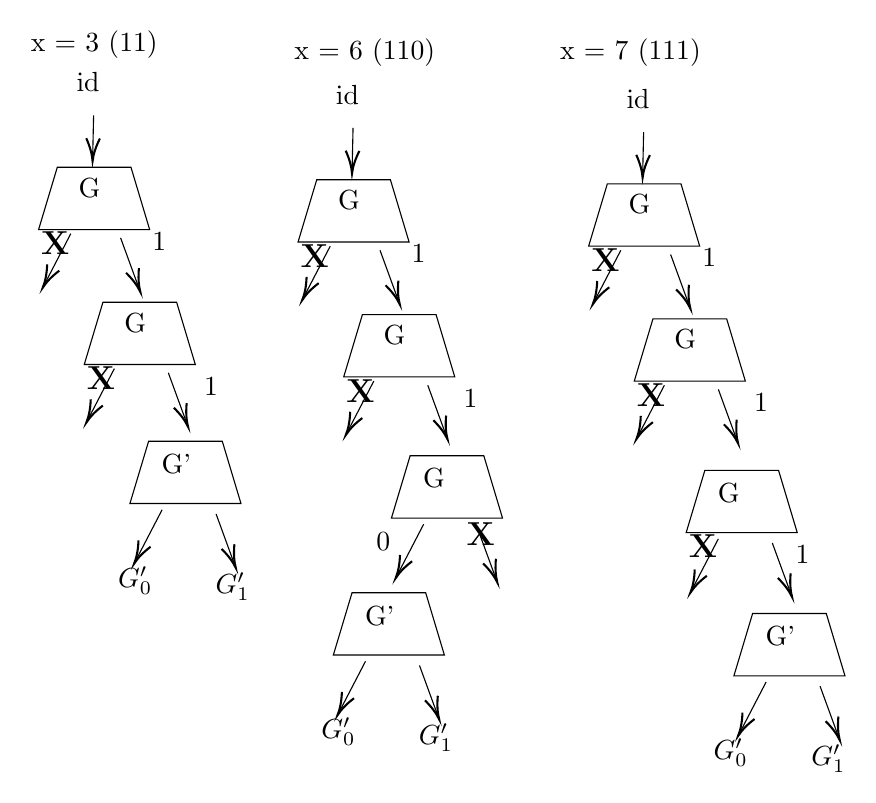
\begin{tikzpicture}[x=0.75pt,y=0.75pt,yscale=-1,xscale=1]
%uncomment if require: \path (0,483); %set diagram left start at 0, and has height of 483

%Shape: Trapezoid [id:dp2852104231671544]
\draw   (45,120) -- (54,90) -- (89.5,90) -- (98.5,120) -- cycle ;
%Shape: Trapezoid [id:dp165141673263979]
\draw   (67,185) -- (76,155) -- (111.5,155) -- (120.5,185) -- cycle ;
%Straight Lines [id:da29030255403190575]
\draw    (107.5,189) -- (116.31,213.12) ;
\draw [shift={(117,215)}, rotate = 249.93] [color={rgb, 255:red, 0; green, 0; blue, 0 }  ][line width=0.75]    (10.93,-3.29) .. controls (6.95,-1.4) and (3.31,-0.3) .. (0,0) .. controls (3.31,0.3) and (6.95,1.4) .. (10.93,3.29)   ;
%Straight Lines [id:da9510990729773141]
\draw    (84.5,124) -- (93.31,148.12) ;
\draw [shift={(94,150)}, rotate = 249.93] [color={rgb, 255:red, 0; green, 0; blue, 0 }  ][line width=0.75]    (10.93,-3.29) .. controls (6.95,-1.4) and (3.31,-0.3) .. (0,0) .. controls (3.31,0.3) and (6.95,1.4) .. (10.93,3.29)   ;
%Straight Lines [id:da0037293976213679247]
\draw    (60.5,122) -- (47.92,146.23) ;
\draw [shift={(47,148)}, rotate = 297.44] [color={rgb, 255:red, 0; green, 0; blue, 0 }  ][line width=0.75]    (10.93,-3.29) .. controls (6.95,-1.4) and (3.31,-0.3) .. (0,0) .. controls (3.31,0.3) and (6.95,1.4) .. (10.93,3.29)   ;
%Straight Lines [id:da8228080900603938]
\draw    (81.5,187) -- (68.92,211.23) ;
\draw [shift={(68,213)}, rotate = 297.44] [color={rgb, 255:red, 0; green, 0; blue, 0 }  ][line width=0.75]    (10.93,-3.29) .. controls (6.95,-1.4) and (3.31,-0.3) .. (0,0) .. controls (3.31,0.3) and (6.95,1.4) .. (10.93,3.29)   ;
%Straight Lines [id:da28500051662317105]
\draw    (71.5,65) -- (71.05,85) ;
\draw [shift={(71,87)}, rotate = 271.3] [color={rgb, 255:red, 0; green, 0; blue, 0 }  ][line width=0.75]    (10.93,-3.29) .. controls (6.95,-1.4) and (3.31,-0.3) .. (0,0) .. controls (3.31,0.3) and (6.95,1.4) .. (10.93,3.29)   ;
%Shape: Trapezoid [id:dp6325112610108554]
\draw   (170,126) -- (179,96) -- (214.5,96) -- (223.5,126) -- cycle ;
%Shape: Trapezoid [id:dp25188600140982165]
\draw   (192,191) -- (201,161) -- (236.5,161) -- (245.5,191) -- cycle ;
%Shape: Trapezoid [id:dp7252358609087375]
\draw   (215,259) -- (224,229) -- (259.5,229) -- (268.5,259) -- cycle ;
%Straight Lines [id:da7972073805415487]
\draw    (232.5,195) -- (241.31,219.12) ;
\draw [shift={(242,221)}, rotate = 249.93] [color={rgb, 255:red, 0; green, 0; blue, 0 }  ][line width=0.75]    (10.93,-3.29) .. controls (6.95,-1.4) and (3.31,-0.3) .. (0,0) .. controls (3.31,0.3) and (6.95,1.4) .. (10.93,3.29)   ;
%Straight Lines [id:da018853121174194687]
\draw    (209.5,130) -- (218.31,154.12) ;
\draw [shift={(219,156)}, rotate = 249.93] [color={rgb, 255:red, 0; green, 0; blue, 0 }  ][line width=0.75]    (10.93,-3.29) .. controls (6.95,-1.4) and (3.31,-0.3) .. (0,0) .. controls (3.31,0.3) and (6.95,1.4) .. (10.93,3.29)   ;
%Straight Lines [id:da7054896933784254]
\draw    (185.5,128) -- (172.92,152.23) ;
\draw [shift={(172,154)}, rotate = 297.44] [color={rgb, 255:red, 0; green, 0; blue, 0 }  ][line width=0.75]    (10.93,-3.29) .. controls (6.95,-1.4) and (3.31,-0.3) .. (0,0) .. controls (3.31,0.3) and (6.95,1.4) .. (10.93,3.29)   ;
%Straight Lines [id:da18444998536360768]
\draw    (206.5,193) -- (193.92,217.23) ;
\draw [shift={(193,219)}, rotate = 297.44] [color={rgb, 255:red, 0; green, 0; blue, 0 }  ][line width=0.75]    (10.93,-3.29) .. controls (6.95,-1.4) and (3.31,-0.3) .. (0,0) .. controls (3.31,0.3) and (6.95,1.4) .. (10.93,3.29)   ;
%Straight Lines [id:da255539280729278]
\draw    (196.5,71) -- (196.05,91) ;
\draw [shift={(196,93)}, rotate = 271.3] [color={rgb, 255:red, 0; green, 0; blue, 0 }  ][line width=0.75]    (10.93,-3.29) .. controls (6.95,-1.4) and (3.31,-0.3) .. (0,0) .. controls (3.31,0.3) and (6.95,1.4) .. (10.93,3.29)   ;
%Straight Lines [id:da9761312714264434]
\draw    (256.5,264) -- (265.31,288.12) ;
\draw [shift={(266,290)}, rotate = 249.93] [color={rgb, 255:red, 0; green, 0; blue, 0 }  ][line width=0.75]    (10.93,-3.29) .. controls (6.95,-1.4) and (3.31,-0.3) .. (0,0) .. controls (3.31,0.3) and (6.95,1.4) .. (10.93,3.29)   ;
%Straight Lines [id:da6224568075589378]
\draw    (230.5,262) -- (217.92,286.23) ;
\draw [shift={(217,288)}, rotate = 297.44] [color={rgb, 255:red, 0; green, 0; blue, 0 }  ][line width=0.75]    (10.93,-3.29) .. controls (6.95,-1.4) and (3.31,-0.3) .. (0,0) .. controls (3.31,0.3) and (6.95,1.4) .. (10.93,3.29)   ;
%Shape: Trapezoid [id:dp6872434343845957]
\draw   (310,128) -- (319,98) -- (354.5,98) -- (363.5,128) -- cycle ;
%Shape: Trapezoid [id:dp5707224683508241]
\draw   (332,193) -- (341,163) -- (376.5,163) -- (385.5,193) -- cycle ;
%Straight Lines [id:da12843330917593843]
\draw    (372.5,197) -- (381.31,221.12) ;
\draw [shift={(382,223)}, rotate = 249.93] [color={rgb, 255:red, 0; green, 0; blue, 0 }  ][line width=0.75]    (10.93,-3.29) .. controls (6.95,-1.4) and (3.31,-0.3) .. (0,0) .. controls (3.31,0.3) and (6.95,1.4) .. (10.93,3.29)   ;
%Straight Lines [id:da4469168554714653]
\draw    (349.5,132) -- (358.31,156.12) ;
\draw [shift={(359,158)}, rotate = 249.93] [color={rgb, 255:red, 0; green, 0; blue, 0 }  ][line width=0.75]    (10.93,-3.29) .. controls (6.95,-1.4) and (3.31,-0.3) .. (0,0) .. controls (3.31,0.3) and (6.95,1.4) .. (10.93,3.29)   ;
%Straight Lines [id:da7422932295865028]
\draw    (325.5,130) -- (312.92,154.23) ;
\draw [shift={(312,156)}, rotate = 297.44] [color={rgb, 255:red, 0; green, 0; blue, 0 }  ][line width=0.75]    (10.93,-3.29) .. controls (6.95,-1.4) and (3.31,-0.3) .. (0,0) .. controls (3.31,0.3) and (6.95,1.4) .. (10.93,3.29)   ;
%Straight Lines [id:da4132308539243472]
\draw    (346.5,195) -- (333.92,219.23) ;
\draw [shift={(333,221)}, rotate = 297.44] [color={rgb, 255:red, 0; green, 0; blue, 0 }  ][line width=0.75]    (10.93,-3.29) .. controls (6.95,-1.4) and (3.31,-0.3) .. (0,0) .. controls (3.31,0.3) and (6.95,1.4) .. (10.93,3.29)   ;
%Straight Lines [id:da772807844960463]
\draw    (336.5,73) -- (336.05,93) ;
\draw [shift={(336,95)}, rotate = 271.3] [color={rgb, 255:red, 0; green, 0; blue, 0 }  ][line width=0.75]    (10.93,-3.29) .. controls (6.95,-1.4) and (3.31,-0.3) .. (0,0) .. controls (3.31,0.3) and (6.95,1.4) .. (10.93,3.29)   ;
%Shape: Trapezoid [id:dp46398684125614054]
\draw   (357,266) -- (366,236) -- (401.5,236) -- (410.5,266) -- cycle ;
%Straight Lines [id:da11861488343609228]
\draw    (398.5,271) -- (407.31,295.12) ;
\draw [shift={(408,297)}, rotate = 249.93] [color={rgb, 255:red, 0; green, 0; blue, 0 }  ][line width=0.75]    (10.93,-3.29) .. controls (6.95,-1.4) and (3.31,-0.3) .. (0,0) .. controls (3.31,0.3) and (6.95,1.4) .. (10.93,3.29)   ;
%Straight Lines [id:da9516374594621448]
\draw    (372.5,269) -- (359.92,293.23) ;
\draw [shift={(359,295)}, rotate = 297.44] [color={rgb, 255:red, 0; green, 0; blue, 0 }  ][line width=0.75]    (10.93,-3.29) .. controls (6.95,-1.4) and (3.31,-0.3) .. (0,0) .. controls (3.31,0.3) and (6.95,1.4) .. (10.93,3.29)   ;
%Shape: Trapezoid [id:dp08951129262323287]
\draw   (380,335) -- (389,305) -- (424.5,305) -- (433.5,335) -- cycle ;
%Straight Lines [id:da7484649651346909]
\draw    (421.5,340) -- (430.31,364.12) ;
\draw [shift={(431,366)}, rotate = 249.93] [color={rgb, 255:red, 0; green, 0; blue, 0 }  ][line width=0.75]    (10.93,-3.29) .. controls (6.95,-1.4) and (3.31,-0.3) .. (0,0) .. controls (3.31,0.3) and (6.95,1.4) .. (10.93,3.29)   ;
%Straight Lines [id:da33509456958885586]
\draw    (395.5,338) -- (382.92,362.23) ;
\draw [shift={(382,364)}, rotate = 297.44] [color={rgb, 255:red, 0; green, 0; blue, 0 }  ][line width=0.75]    (10.93,-3.29) .. controls (6.95,-1.4) and (3.31,-0.3) .. (0,0) .. controls (3.31,0.3) and (6.95,1.4) .. (10.93,3.29)   ;
%Shape: Trapezoid [id:dp32493714209065194]
\draw   (187,325) -- (196,295) -- (231.5,295) -- (240.5,325) -- cycle ;
%Straight Lines [id:da9049293232409525]
\draw    (228.5,330) -- (237.31,354.12) ;
\draw [shift={(238,356)}, rotate = 249.93] [color={rgb, 255:red, 0; green, 0; blue, 0 }  ][line width=0.75]    (10.93,-3.29) .. controls (6.95,-1.4) and (3.31,-0.3) .. (0,0) .. controls (3.31,0.3) and (6.95,1.4) .. (10.93,3.29)   ;
%Straight Lines [id:da2546698999144019]
\draw    (202.5,328) -- (189.92,352.23) ;
\draw [shift={(189,354)}, rotate = 297.44] [color={rgb, 255:red, 0; green, 0; blue, 0 }  ][line width=0.75]    (10.93,-3.29) .. controls (6.95,-1.4) and (3.31,-0.3) .. (0,0) .. controls (3.31,0.3) and (6.95,1.4) .. (10.93,3.29)   ;
%Shape: Trapezoid [id:dp28639357131974275]
\draw   (89,252) -- (98,222) -- (133.5,222) -- (142.5,252) -- cycle ;
%Straight Lines [id:da7386120130934712]
\draw    (130.5,257) -- (139.31,281.12) ;
\draw [shift={(140,283)}, rotate = 249.93] [color={rgb, 255:red, 0; green, 0; blue, 0 }  ][line width=0.75]    (10.93,-3.29) .. controls (6.95,-1.4) and (3.31,-0.3) .. (0,0) .. controls (3.31,0.3) and (6.95,1.4) .. (10.93,3.29)   ;
%Straight Lines [id:da9354417450920047]
\draw    (104.5,255) -- (91.92,279.23) ;
\draw [shift={(91,281)}, rotate = 297.44] [color={rgb, 255:red, 0; green, 0; blue, 0 }  ][line width=0.75]    (10.93,-3.29) .. controls (6.95,-1.4) and (3.31,-0.3) .. (0,0) .. controls (3.31,0.3) and (6.95,1.4) .. (10.93,3.29)   ;

% Text Node
\draw (62,43) node [anchor=north west][inner sep=0.75pt]   [align=left] {id};
% Text Node
\draw (63,94) node [anchor=north west][inner sep=0.75pt]   [align=left] {G};
% Text Node
\draw (85,159) node [anchor=north west][inner sep=0.75pt]   [align=left] {G};
% Text Node
\draw (67,185) node [anchor=north west][inner sep=0.75pt]   [align=left] {\textbf{{\large X}}};
% Text Node
\draw (45,120) node [anchor=north west][inner sep=0.75pt]   [align=left] {\textbf{{\large X}}};
% Text Node
\draw (40,23) node [anchor=north west][inner sep=0.75pt]   [align=left] {x = 3 (11)};
% Text Node
\draw (98.5,120) node [anchor=north west][inner sep=0.75pt]   [align=left] {1};
% Text Node
\draw (123.5,190) node [anchor=north west][inner sep=0.75pt]   [align=left] {1};
% Text Node
\draw (187,49) node [anchor=north west][inner sep=0.75pt]   [align=left] {id};
% Text Node
\draw (188,100) node [anchor=north west][inner sep=0.75pt]   [align=left] {G};
% Text Node
\draw (210,165) node [anchor=north west][inner sep=0.75pt]   [align=left] {G};
% Text Node
\draw (229,234) node [anchor=north west][inner sep=0.75pt]   [align=left] {G};
% Text Node
\draw (192,191) node [anchor=north west][inner sep=0.75pt]   [align=left] {\textbf{{\large X}}};
% Text Node
\draw (170,126) node [anchor=north west][inner sep=0.75pt]   [align=left] {\textbf{{\large X}}};
% Text Node
\draw (167,27) node [anchor=north west][inner sep=0.75pt]   [align=left] {x = 6 (110)};
% Text Node
\draw (223.5,126) node [anchor=north west][inner sep=0.75pt]   [align=left] {1};
% Text Node
\draw (248.5,196) node [anchor=north west][inner sep=0.75pt]   [align=left] {1};
% Text Node
\draw (206.5,265) node [anchor=north west][inner sep=0.75pt]   [align=left] {0};
% Text Node
\draw (295,27) node [anchor=north west][inner sep=0.75pt]   [align=left] {x = 7 (111)};
% Text Node
\draw (250,260) node [anchor=north west][inner sep=0.75pt]   [align=left] {\textbf{{\large X}}};
% Text Node
\draw (327,51) node [anchor=north west][inner sep=0.75pt]   [align=left] {id};
% Text Node
\draw (328,102) node [anchor=north west][inner sep=0.75pt]   [align=left] {G};
% Text Node
\draw (350,167) node [anchor=north west][inner sep=0.75pt]   [align=left] {G};
% Text Node
\draw (332,193) node [anchor=north west][inner sep=0.75pt]   [align=left] {\textbf{{\large X}}};
% Text Node
\draw (310,128) node [anchor=north west][inner sep=0.75pt]   [align=left] {\textbf{{\large X}}};
% Text Node
\draw (363.5,128) node [anchor=north west][inner sep=0.75pt]   [align=left] {1};
% Text Node
\draw (388.5,198) node [anchor=north west][inner sep=0.75pt]   [align=left] {1};
% Text Node
\draw (371,241) node [anchor=north west][inner sep=0.75pt]   [align=left] {G};
% Text Node
\draw (357,266) node [anchor=north west][inner sep=0.75pt]   [align=left] {\textbf{{\large X}}};
% Text Node
\draw (394,310) node [anchor=north west][inner sep=0.75pt]   [align=left] {G'};
% Text Node
\draw (408.5,271) node [anchor=north west][inner sep=0.75pt]   [align=left] {1};
% Text Node
\draw (201,300) node [anchor=north west][inner sep=0.75pt]   [align=left] {G'};
% Text Node
\draw (180,354) node [anchor=north west][inner sep=0.75pt]    {$G'_{0}$};
% Text Node
\draw (227,357) node [anchor=north west][inner sep=0.75pt]    {$G'_{1}$};
% Text Node
\draw (369,364) node [anchor=north west][inner sep=0.75pt]    {$G'_{0}$};
% Text Node
\draw (416,367) node [anchor=north west][inner sep=0.75pt]    {$G'_{1}$};
% Text Node
\draw (103,227) node [anchor=north west][inner sep=0.75pt]   [align=left] {G'};
% Text Node
\draw (82,281) node [anchor=north west][inner sep=0.75pt]    {$G'_{0}$};
% Text Node
\draw (129,284) node [anchor=north west][inner sep=0.75pt]    {$G'_{1}$};


\end{tikzpicture}

  Evaluating with $x=11 (3)$ will give us $g_{id}(11) = $($G'_0(G_1(G_1(id)))$,   $G'_1(G_1(G_1(id)))$). For ease of explanation, I will refer to $a = G'_0(G_1(G_1(id)))$ and $b = G'_1(G_1(G_1(id)))$

  Then, evaluating with $x=110 (6)$ will give us $g_{id}(110) = $($G'_0(a)$,   $G'_1(a)$). \newline
  The Goldreich-Levin hardcore predicate theorem states that, if you have a OWP $g_{id}$, the output looks random, and is unpredictable. However, since we have the input and output of $G'$ at an input $a$, we know what $G'$ does. $G'$ has been compromised. We can predict the output of the PRG $G'$. \newline

  Finally, let's evaluate with $x=111 (7)$. The GGM construction gives is $g_{id}(111) = $($G_0(b)$,   $G'_1(b)$). Since we have compromised $G'$ and know what it does, we can predict this output. This means that the PRFF is NOT SECURE.

    }
%%%%%%%%%%%%%%%%%%
     \newpage


%%%%%%%%%%%%%%%%%%%%%%%%%%%%%%%%%%%%%%%%%%%%%%%%%%
%%%%%%%%%%%% PROBLEM 4 %%%%%%%%%%%%%%%%%%%%%%%%%%%%
%%%%%%%%%%%%%%%%%%%%%%%%%%%%%%%%%%%%%%%%%%%%%%%%%%%
\item {\bfseries OWF.} (10 points)
Let $f:\{0,1\}^n \rightarrow \{0,1\}^n$ be a one-way function. Define
$g: \{0,1\}^{2n}\rightarrow \{0,1\}^{2n}$ as \[g(x_1,x_2)=f(x_2)||x_1\oplus x_2 \oplus 1^n\]\\
where $x_1 \in \{0,1\}^n$, $x_2 \in \{0,1\}^n$ and $1^n$ denotes a string of $n$ bits. Show that $g$ is also a one-way function. \newline 
{\footnotesize Hint. Suppose there exists an efficient adversary $\cA$ that inverts the function $g$ . 
  You should now construct a new efficient adversary $\cA'$ that uses $\cA$ as a subroutine to invert the function $f$.} \newline 
%%%%% ANSWER %%%%%
    {\bfseries

    Let's suppose that $g$ is NOT a OWF, and the efficient adversary $\cA$ knows how to invert $g$. \newline

    Now, let's say that $f(x_2)$ is given to the efficient adversary $\cA'$. $\cA'$ takes $f(x_2)$ and creates a new bit string $y$ to give to the efficient adversary $\cA$. $y$ should be the output of $g(x_1, x_2)$. The bit string $y = f(x_2) || $<random n bits>. The first $n$ bits of $y$ will be $f(x_2)$, since that's how $g$ is defined. The last $n$ bits of $y$ can be anything because $x_1 \oplus x_2 \oplus 1^n$ can result in anything, even with $x_2$ fixed at some value. \newline

    Now, we give $\cA$ the bit string $y$, and since it knows how to invert $g$, it returns an $(x_1, x_2)$ that satisfies $g(x_1, x_2) = y$. \newline

    Since $\cA'$ now knows $x_2$, it returns that, successfully inverting $f$. Since $\cA'$ has inverted $f$, this implies that $f$ is not a OWF, which is a contradiction of what we were told. Therefore, by contradiction, $g$ is also a OWF.
    }
%%%%%%%%%%%%%%%%%%
     \newpage




%%%%%%%%%%%%%%%%%%%%%%%%%%%%%%%%%%%%%%%%%%%%%%%%%%
%%%%%%%%%%%% PROBLEM 5 %%%%%%%%%%%%%%%%%%%%%%%%%%%%
%%%%%%%%%%%%%%%%%%%%%%%%%%%%%%%%%%%%%%%%%%%%%%%%%%%
\item {\bfseries Encryption using Random Functions.} (15+10 points)
  Let $\cF$ be the set of all functions $\zo^{n} \to \zo^n$. 
  Consider the following private-key encryption scheme. 
  \begin{boxedalgo}
  \begin{itemize}
  \item $\gen()$: Return $\sk=F$ uniformly at random from the set $\cF$ 
  \item $\enc_\sk(m)$: Return $(c,r)$, where $r$ is chosen uniformly at random from $\zo^n$, $c = m\oplus F(r)$, and $\sk=F$.  
  \item $\dec_\sk(\widetilde c,\widetilde r)$: Return $\widetilde c \oplus F(\widetilde r)$.
  \end{itemize}
  \end{boxedalgo}
  
  \begin{enumerate}
  \item (15 points) Suppose we want to ensure that even if we make $10^{10}$ calls to the encryption algorithm, all randomness $r$ that are chosen are distinct with probability $1-2^{- 201}$. 
    What value of $n$ shall you choose? \newline 
%%%%% ANSWER %%%%%
    {\bfseries
      For a sample size $S$:

      $S = \{0,1\}^n$, and $|S| = 2^n$ \newline

      And if we pick a sample from the set $S$ $K = 10^{10}$ times, we would like the probability that all samples are distinct with probability at least $1-2^{-201}$. \newline

      We first recall that, for a sample space, $\P$[K samples distinct]$\approx exp(\frac{-K^2}{2*|S|})$ \newline

      It follows that: \newline

      $exp(\frac{-K^2}{2*|S|})$ \newline
      $exp(\frac{-10^{20}}{2*2^n})$ \newline
      $exp(\frac{-10^{20}}{2^{n+1}})$ \newline

      Remembering that $1-2^{-201} \approx exp(2^{-201})$, We now must ensure that:
      $exp(\frac{-10^{20}}{2^{n+1}}) \geq exp(-2^{-201})$ \newline
      $\frac{-10^{20}}{2^{n+1}} \geq -2^{-201}$ \newline
      $\frac{10^{20}}{2^{n+1}} \leq 2^{-201}$ \newline
      $ 10^{20} \leq 2^{n-200}$ \newline
      $n \geq \frac{20*\ln{10}}{\ln{2}} + 200$ \newline
      $n \geq 266.438$ \newline

      And since $n$ must be an integer, we round it up to $267$. Therefore, if we would like to make $10^{10}$ calls to the encryption algorithm, we can ensure that all randomness $r$ that are chosen are distinct with probability at least $1-2^{-201}$ by using a value of $n=267$.

    }
%%%%%%%%%%%%%%%%%%
     \newpage

  \item (10 points) Conditioned on the fact that all randomness $r$ in the encryption schemes are distinct, prove that this scheme is secure. \newline 
%%%%% ANSWER %%%%%
    {\bfseries
      This scheme is similar to one-time pad. We already know that one-time pad is perfectly secure with a secret key that cannot be computed by any adversary. \newline

      In order for us to say that this scheme is secure we must prove that $F(r)$ is completely unpredictable and random for every $r$.  \newline


      The definition of a random function states the following: \newline

      Choose any $x_1 \in \D$. \newline
      $F(x_1)$ is uniformly random over $\R$, and now we know that $F(x_1) = y_1$. \newline

      Now, choose any $x_2 \in \D$. \newline
      If $x_2 = x_1$, then $F(x_1) = F(x_2)$. Otherwise, $F(x_2)$ is uniformly random over $\R$. \newline

      This means that, for any input given to $F$ that you haven't seen the output, it is COMPLTELY IMPOSSIBLE to predict the output. Furthermore, since every randomness $r$ given to $F$ will be unique (for every input, we have never seen the output), we can confidently say that the output of $F$ will always be completely unpredictable and random. No adversary will be able to compute the secret key.

      Since one-time pad is perfectly secure with a completely random, uncomputable secret key, we can conclude that this scheme is secure.
    }
%%%%%%%%%%%%%%%%%%
     \newpage

  \end{enumerate}
 

%%%%%%%%%%%%%%%%%%%%%%%%%%%%%%%%%%%%%%%%%%%%%%%%%%
%%%%%%%%%%%% PROBLEM 6 %%%%%%%%%%%%%%%%%%%%%%%%%%%%
%%%%%%%%%%%%%%%%%%%%%%%%%%%%%%%%%%%%%%%%%%%%%%%%%%%
\item {\bfseries Birthday Paradox.} (10 points)   
Recall that the Birthday Paradox states that if we throw $m= c\sqrt{n}$ balls into $n$ bins, then the probability that there exists a collision (\ie, a bin with at least two balls) is $\geq 0.99$, where $c>0$ is an appropriate constant. \newline
An international university has 12 colleges. Moreover, the students of this university come from 100 different countries around the world. How many students (from the university) in a room will ensure with probability $\geq 0.99$ that there exists at
least a pair of students such that they are from the same country, the same college, and they celebrate their birthday at the same month.
%%%%% ANSWER %%%%%
    {\bfseries

    We should think of the number of students $m$ as balls, $m=c \sqrt n$. \newline

    We should also think of the number of bins $n$ as the possible combinations of colleges, countries, and months. Given that there are 12 different colleges, 100 different countries, and 12 different months, it follows that there are a total of $12*12*100 = 14,400$ possible combinations of those three, so there are 14,400 bins. \newline

    So, $n = 14,400$ \newline
    and $m = c\sqrt n = c\sqrt{14,400} = 120c$ \newline

    Therefore, you just need $120c$ students in a room to ensure with probability $\geq 0.99$ that there exists at least one pair of students such that they are from the same country, the same college, and they celebrate their birthday at the same month.
    }
%%%%%%%%%%%%%%%%%%
\newpage


%%%%%%%%%%%%%%%%%%%%%%%%%%%%%%%%%%%%%%%%%%%%%%%%%%
%%%%%%%%%%%% PROBLEM 7 %%%%%%%%%%%%%%%%%%%%%%%%%%%%
%%%%%%%%%%%%%%%%%%%%%%%%%%%%%%%%%%%%%%%%%%%%%%%%%%%
\item
{\bfseries PRF.}(10 points) 
Suppose the set of functions $F_\id \colon \zo^n\to\zo^n$ forms a \ul{secure} PRF when $\id$ is chosen uniformly at random from the set $\zo^n$.

We are now constructing a new PRF family $G_\id\colon\zo^{2n}\to\zo^{2n}$, where $\id\in\zo^n$. 
This new function is defined as follows.
  $$ G_\id(x_1,x_2) \defeq \left( ~  x_2 \xor F_\id(x_1) ~, ~ F_\id(x_2) ~ \right)$$
Is this new PRF secure or not? 

(If you think that it is secure, then prove that it is secure.
If you think that it is insecure, then prove why this construction is insecure. 
You get no points for just writing Yes/No.)

%%%%% ANSWER %%%%%
    {\bfseries
    I do not think this PRF is secure. An adversary will notice that, whatever the value of $x_2$, the output of $G_{id}(x_1, x_2)$ ends in whatever $F_{id}(x_2)$ evaluates to (the last $n$ bits).\newline

    Using this, we can predict the output for some combination of $(x_1, x_2)$ that has not been seen before. Here's a simple example: \newline

    Input to $G_{id} = 001$ $010$ \newline
    $G_{id}(001, 010) = ( 010 \xor F_{id}(001), F_{id}(010) )$ \newline
    We know that the last $n$ bits of $G_{id}(001, 010) = F_{id}(010)$. \newline

    Input to $G_id = 010$ $010$ \newline
    We know $x_2 = 010$ because we chose it, and we know $F_{id}(x_1) = F_{id}(010)$ from the previous input we evaluated. Therefore, we can predict the following equation, since we know all parts of it. \newline
    $G_{id}(010, 010) = ( 010 \xor F_{id}(010), F_{id}(010) )$ \newline

    Even though $F_{id}$ itself is secure, this example shows a way that you can predict output for a PRF. This proves that $G_{id}$ is NOT secure.
    }
%%%%%%%%%%%%%%%%%%


\newpage
\end{enumerate}
%%%%%%%%%%%%%%%%%%%%%%%%%%%%%%%%%%%%%%%%%%%%%%%%%%
%%%%%%%%%%%% PLEASE LIST COLLABORATORS BELOW  %%%%%
%%%%%%%%%%%%%%%%%%%%%%%%%%%%%%%%%%%%%%%%%%%%%%%%%%%
{\bfseries Collaborators :} \newline 
% ENTER THEIR NAMES HERE  

\end{document}
